\subsection{Метрика Махаланобис}

    Как было показано выше значение критической интенсивности, а значит и вероятности выживания популяции зависит от двух факторов: стохастической чувствительности аттрактора и расстояния до границы бассейна притяжения. Метрика Махаланобиса показывает расстояние между двумя точками с учетом стохастической чувствительности аттрактора.

    Метрика Махаланобис рассчитывается по формуле:

    \[
        d_M = \frac{|x_2^* - x_1^*|}{\sqrt{M}},
    \]
        
    где \(x_2^*\) --- устойчивое равновесие, либо один из элементов цикла, либо граница хаотического аттрактора, а \(x_1^*\) --- либо неустойчивое равновесие, либо его прообраз, \(M\) --- значение функции стохастической чувствительности.

    Графики зависимостей метрики Махаланобиса от параметра \(\beta\) изображены на рисунках \ref{mahalanobis_metrics_alpha_noise}, \ref{mahalanobis_metrics_beta_noise} и \ref{mahalanobis_metrics_additive_noise}. Аналогично на рисунках \ref{euclid_metrics_alpha_noise}, \ref{euclid_metrics_beta_noise} и \ref{euclid_metrics_additive_noise} изображены графики зависимостей евклидовой метрики от параметра \(\beta\).

    % \vspace{\abovedisplayskip}
    \begin{figure}
        \begin{minipage}{0.45\textwidth}
            \centering
            \subfloat[Для модели (\ref{alpha_chaos}) (\(\alpha\)-шум)]{
                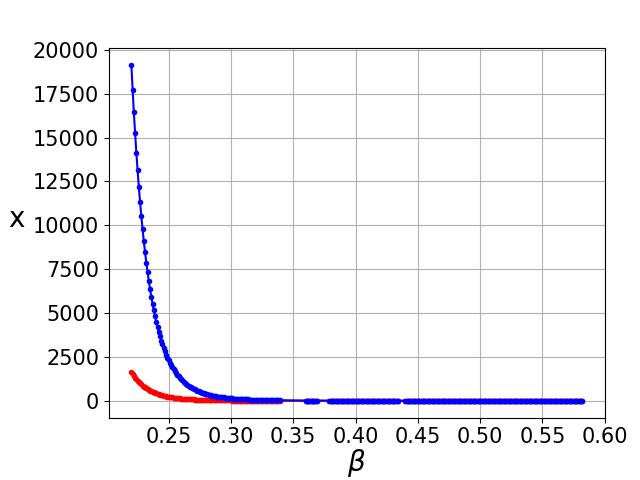
\includegraphics[width=\textwidth]{stochastic/images/mahalanobis_metrics_alpha_noise.jpg}
                \label{mahalanobis_metrics_alpha_noise}
            }
        
            \subfloat[Для модели (\ref{beta_chaos}) (\(\beta\)-шум)]{
                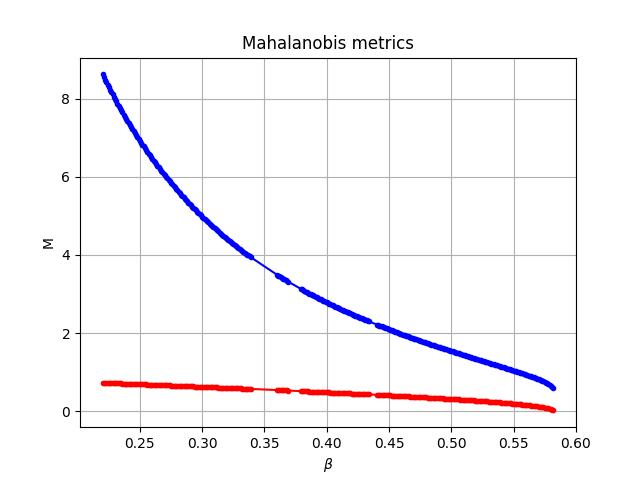
\includegraphics[width=\textwidth]{stochastic/images/mahalanobis_metrics_beta_noise.jpg}
                \label{mahalanobis_metrics_beta_noise}
            }  
        
            \subfloat[Для модели (\ref{additive_chaos}) (аддитивный шум)]{
                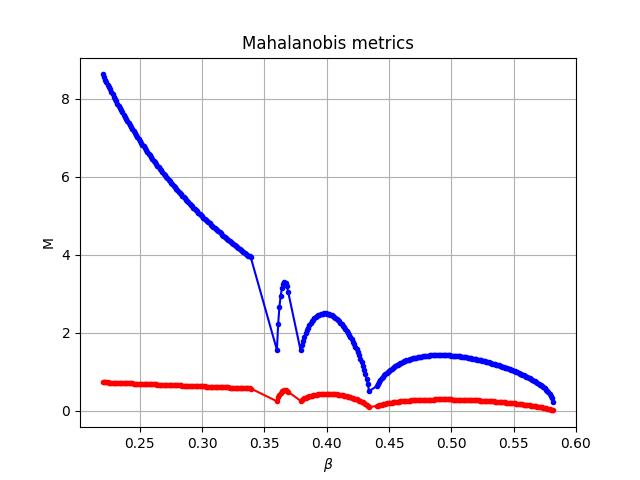
\includegraphics[width=\textwidth]{stochastic/images/mahalanobis_metrics_additive_noise.jpg}
                \label{mahalanobis_metrics_additive_noise}
            }
                
            \captionsetup{justification=centering}
            \caption{Метрика Махаланобис}
        \end{minipage}
        \hfill
        \begin{minipage}{0.45\textwidth}
            \centering
            \subfloat[Для модели (\ref{alpha_chaos}) (\(\alpha\)-шум)]{
                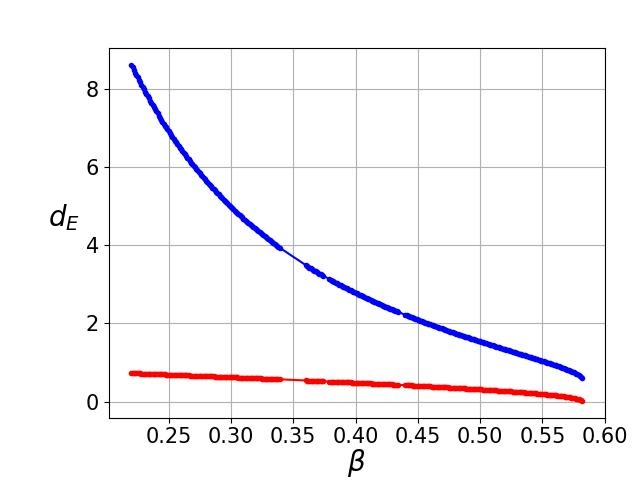
\includegraphics[width=\textwidth]{stochastic/images/euclid_metrics_alpha_noise.jpg}
                \label{euclid_metrics_alpha_noise}
            }
            
            \subfloat[Для модели (\ref{beta_chaos}) (\(\beta\)-шум)]{
                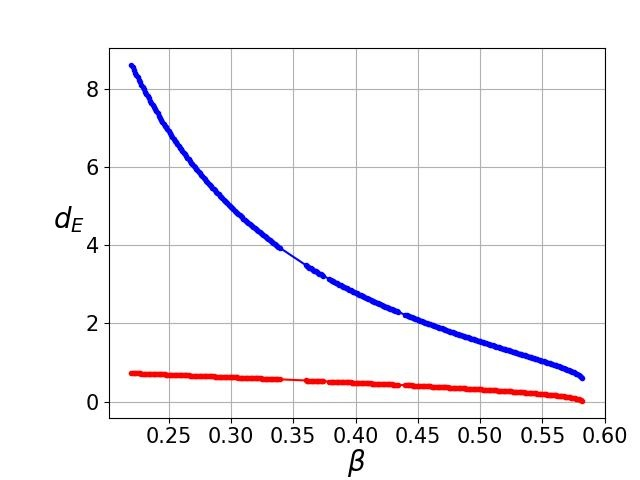
\includegraphics[width=\textwidth]{stochastic/images/euclid_metrics_beta_noise.jpg}
                \label{euclid_metrics_beta_noise}
            }  
    
            \subfloat[Для модели (\ref{additive_chaos}) (аддитивный шум)]{
                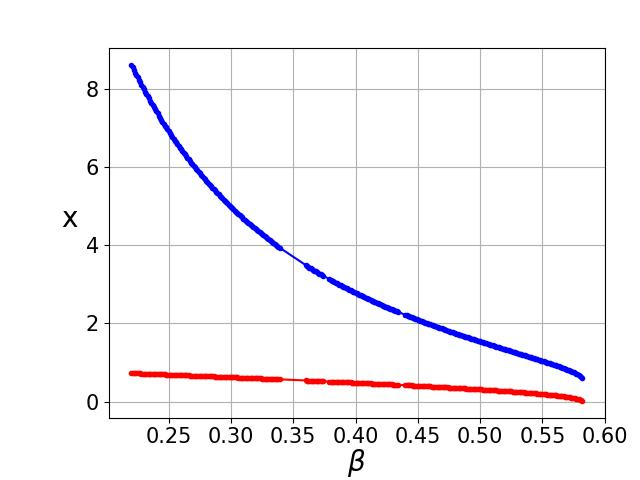
\includegraphics[width=\textwidth]{stochastic/images/euclid_metrics_additive_noise.jpg}
                \label{euclid_metrics_additive_noise}
            }
            
            \captionsetup{justification=centering}
            \caption{Евклидова метрика}
        \end{minipage}
    \end{figure}
    % \vspace{\abovedisplayskip}

    % \begin{figure}
    %     \centering
    %     \subfloat[Для модели (\ref{alpha_chaos})]{
    %         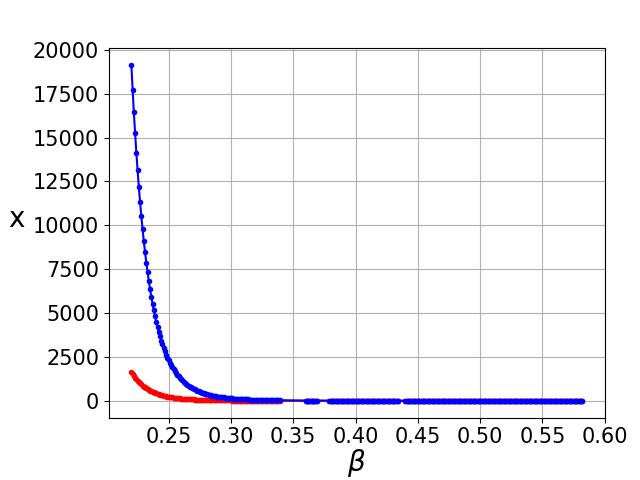
\includegraphics[width=0.55\textwidth]{stochastic/images/mahalanobis_metrics_alpha_noise.jpg}
    %         \label{mahalanobis_metrics_alpha_noise}
    %     }
        
    %     \subfloat[Для модели (\ref{beta_chaos})]{
    %         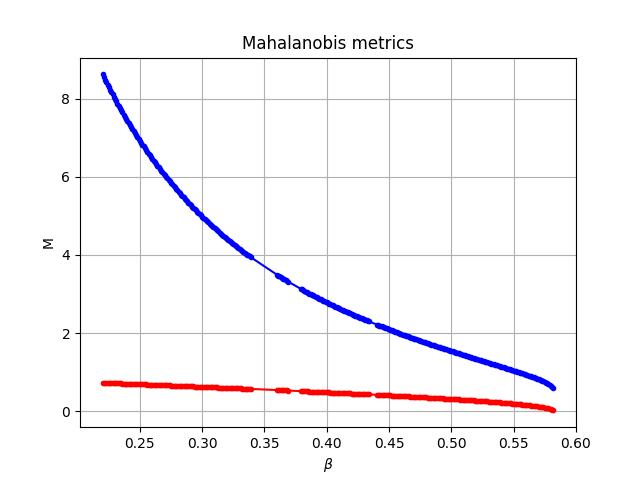
\includegraphics[width=0.55\textwidth]{stochastic/images/mahalanobis_metrics_beta_noise.jpg}
    %         \label{mahalanobis_metrics_beta_noise}
    %     }  

    %     \subfloat[Для модели (\ref{additive_chaos})]{
    %         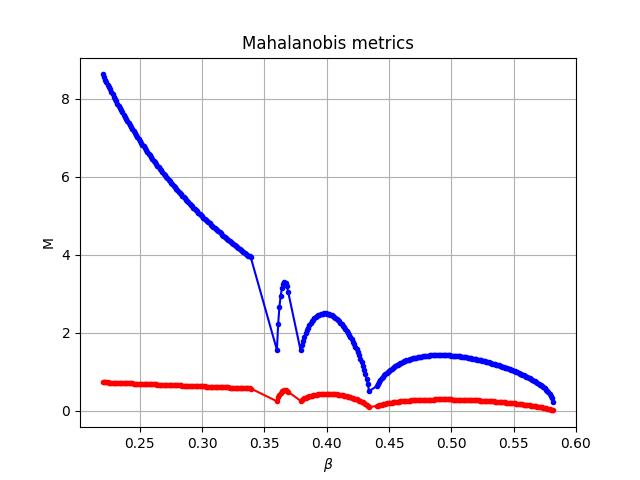
\includegraphics[width=0.55\textwidth]{stochastic/images/mahalanobis_metrics_additive_noise.jpg}
    %         \label{mahalanobis_metrics_additive_noise}
    %     }
        
    %     \caption{Метрика Махаланобис}
    % \end{figure}
            